% !TEX root = ../main.tex

\chapter{绪论}


\section{研究背景与意义}

命名实体识别指的是从文本中识别出重要对象(例如人,组织,地点)的自然语言处理任务\parencite{erdogan2010sequence}。
后面我们将使用NER来指代命名实体识别和分类。NER是信息提取、问答系统、句法分析、机器翻译、
面向语义网的元数据标注等应用领域的重要基础工具,在自然语言处理技术走向实用
化的过程中占有重要地位。

NER任务通常包括两部分:(1)实体边界识别;(2)确定实体类别(人名、地名、机构名或其他)。
英语中的命名实体具有比较明显的形式标志(即实体中的每个词的第一个字母要大写),所以实体边界
识别相对容易,任务的重点是确定实体的类别。和英语相比,汉语命名实体识别任务更加复杂,而且相
对于实体类别标注子任务,实体边界的识别更加困难。


\section{国内外研究进展}


\subsection{基于规则的命名实体识别方法}

基于规则和字典的方法是最初代的命名实体识别使用的方法,这些方法多采用由语言学家通过人工方式,
依据数据集特征构建的特定规则模板或者特殊词典。规则包括关键词、位置词、方位词、中心词、指示词、
统计信息、标点符号等。词典是由特征词构成的词典和外部词典共同组成,外部词典指已有的常识词典。
制定好规则和词典后,通常使用匹配的方式对文本进行处理以实现命名实体识别。

这种方法所训练出来的模型通常过拟合于非常特定的结构化文本语料库,如军事信息集、海军作战报告、并购新闻等。


\subsection{基于统计的命名实体识别方法}

\subsubsection{监督学习方法}

在大型注释语料库上训练的监督学习技术为NER提供了当时最好的结果。著名的监督学习算法
主要包括隐马尔可夫模型(HMM)、决策树、最大熵模型(ME)、支持向量机(SVM)、条件随机场(CRF)。
特别是CRF算法是最有效的NER算法之一。NER需要使用许多前导和滞后的非局部序列训练输出标签的概率,
这使得像CRF这样的判别模型比生成模型更为适合。尽管ME模型放宽了生成模型所做的强独立性假设,但他们存在标签偏差问题,
即模型偏向于输出过渡较少的状态。CRF通过联合考虑所有状态中不同特征的权重来解决这一问题,而不是将状态级别的转移概率归一化。
\parencite{sarawagi2004semi}通过制定半CRF模型改进了现有CRF模型,该模型将标签分配给子序列而不是单个实体,并且没有任何显著的额外计算复杂度。
\parencite{passos2014lexicon}在公共数据上使用他们的词典注入Skip-gram模型来学习高质量的短语向量,并将其插入对数线性CRF系统。
实体分析的联合模型(多任务模型)在单个任务上的结果比单独为NER优化的模型更好。
\parencite{durrett2014joint}开发了一个结构化的CRF模型,该模型通过训练3个任务来提高NER(以及其他实体分析任务)的性能,
例如共指解析(文档内聚类)、命名实体识别(粗语义类型)和实体链接(匹配维基百科实体)。



\subsubsection{半监督学习方法}

\parencite{luo2015joint}提出了JERL(Joint Entity Recognition and Linking)模型,即扩展半CRF模型以捕获NER和实体链接之间的依赖关系。
监督学习方法遇到了障碍,因为可用于学习判别特征的结构化文本是有限的。这催生了半监督学习方法,
它利用了非结构化文本的指数增长量,换句话说,网页以无监督的方式从种子注释语料库中获取上下文信息,即bootstarpping。
\parencite{luo2015joint}提出了一种无监督方法,从大规模未标记数据中创建资源丰富的浓缩特征表示,以有效地训练有监督的NER系统,同时仍保持现有高维半监督解决方案的最新结果。



\subsubsection{无监督学习方法}

无监督学习方法主要是从作为输入词的上下文中生成附加特征以与其他 NER 方法结合使用的手段。
\parencite{lin2009phrase}通过在搜索引擎查询日志的私有数据库上执行 K-means 聚类以使用聚类特征来训练他们的CRF模型,
从而在不使用地名词典的情况下获得了当时最优的结果。无监督学习技术工业应用的一个例外是使用词汇资源的聚类方法,
例如Wordnet以便从Wordnet本身分配命名实体类型。尽管为此目的广泛采用了CRF,但仍有许多关于使用神经网络进行NER的论文。
\parencite{ratinov2009design}在感知机模型中使用了非局部特征、从维基百科中提取的地名词典和类似布朗簇的词表示。由于多层前馈神经网络是通用逼近器,
因此这种神经网络也可以潜在地解决NER任务。


\subsection{基于深度学习的命名实体识别方法}

\subsubsection{卷积神经网络}

卷积神经网络(CNN)可以使用反向传播学习丛单词中提取特征向量表示。使用CNN进行句子建模可以追溯到\parencite{collobert2008unified}。
该工作使用多任务学习来输出对NLP任务的多个预测,如POS标记、块、命名实体标记、语义角色、
语义相似词和一个语言模型。使用一个查找表将每个单词转换为用户定义的维度向量。
因此,通过对每个单词应用查找表,n个单词的输入序列$s_1,s_2,\cdots, s_n$
被转换为一系列向量$ws_1,ws_2, \cdots, ws_n$。
这可以看作是一种原始词嵌入方法,其权值是在网络训练中习得的。
在\parencite{collobert2011natural}中,Collobert扩展了他们的工作,
提出了一个通用的基于CNN的框架来解决过多的NLP任务。

我们定义一个有限词表$\mathcal{D}$,对于词表中的每个单词$w\in \mathcal{D}$,一个$d_{wrd}$维特征向量
表示由查找表层$LT_W(·)$给出:
\begin{equation}
	LT_W(w) = \langle W\rangle _w^1
\end{equation}

其中$W \in \mathbb{R} ^{d_{wrd} \times |\mathcal{D}|}$是要学习的参数矩阵,
$\langle W\rangle _w^1 \in \mathbb{R} ^{d_{wrd}}$是第$W$的第$w$列,$d_{wrd}$词向量大小(用户选择的超参数)。
给定一个由$\mathcal{D}$内的T个词$[w]_1^T$组成的句子序列,
查找表层对序列中的每个单词应用相同的操作,产生以下输出矩阵:

\begin{equation}\label{eq1}
	LT_W([w]_1^T) = \left(\langle W\rangle _{[w]_1}^1, \langle W\rangle _{[w]_2}^1, \cdots, \langle W\rangle _{[w]_T}^1 \right)
\end{equation}

该矩阵则可以被填入后续的神经网络层中。
另外,我们可以考虑将词表示成K个离散特征$w \in \mathcal{D}^1 \times \cdots \times \mathcal{D}^k$,
其中$\mathcal{D}_k$是第$k$个特征的词典。利用参数$W^k \in \mathbb{R} ^{d^k_{wrd} \times |\mathcal{D}^k|}$
将查找表$LT_W(·)$与每个特征关联,其中$d^k_{wrd}\in \mathbb{N}$是一个用户指定的向量维度。
给定一个单词$w$,$d_{wrd}=\sum_k d^k_{wrd}$维的特征向量可以通过链接所有查找表的输出获得。

\begin{equation}
	LT_{W^1, \cdots, W^K}([w]^T_1)
	= \left(
		\begin{matrix}
			\langle W^1 \rangle _{[w_1]_1}^1 & \cdots & \langle W^1 \rangle _{[w_1]_T}^1 \\
			\vdots &  & \vdots \\
			\langle W^K \rangle _{[w_K]_1}^1 & \cdots & \langle W^K \rangle _{[w_K]_T}^1 
		\end{matrix}
	\right)
\end{equation}

单词序列$[w]_1^T$的查找表层的矩阵输出类似于\ref{eq1},但为每个离散特征都加入了额外的行。

\begin{equation}\label{eq2}
	LT_{W^1, \cdots, W^K}(w) = 
		\left(\begin{matrix}
			LT_{W^1}(w_1) \\
			\vdots \\
			LT_{W^K}(w_K)
		\end{matrix}\right) =
		\left(\begin{matrix}
			\langle W^1\rangle _{w_1}^1 \\
			\vdots \\
			\langle W^K\rangle _{w_K}^1
		\end{matrix}\right)
	\end{equation}

查找表中的这些向量特征可以有效地学习字典中单词的特征。
现在,我们想使用这些可训练特征作为输入到可训练特征提取器的其他层,这些层可以表示单词组,然后是句子。

查找表层产生的特征向量需要在神经网络的后续层中进行组合,以产生句子中每个单词的标记决策。
在可变长度序列中为每个元素生成标签(这里,句子是单词序列)是机器学习中的一个标准问题。
考虑两种常用的方法来标记一个单词:窗口方法和(卷积)句子方法。

\paragraph{窗口法}

窗口方法假设分配给单个单词的标签取决于它的上下文(即出现在给定单词之前或之后的单词),
给定要标记的单词,我们考虑这个单词周围的单词的固定大小$k_{sz}$(一个超参数)窗口。
窗口中的每个单词首先通过查找表层\ref{eq1}或者\ref{eq2}生成固定大小$d_{wrd}\times k_{sz}$的词特征矩阵。
该矩阵在将每一列向量拼接后可以视为一个$d_{wrd} k_{sz}$维向量,进而被传到后续的神经网络层中。
第一层网络给出的单词特征窗口可以写为:

\begin{equation}
	f^{1}_{\theta}
	= \langle LT_W( [ w ] ^T_1) \rangle ^{d_{win}}_t
	= \left(
			\begin{matrix}{c}
			\langle W \rangle ^1_{[w]_{t - d_{win} / 2}} \\
			\vdots \\
			\langle W \rangle ^1_{[w]_t} \\
			\vdots \\
			\langle W \rangle ^1_{[w]_{t + d_{win} / 2}}
		\end{matrix}
	\right)
\end{equation}

\subparagraph{线性层}

固定大小的向量$f^{l}_{\theta}$可以穿到一个或多个标准神经网络层中,然后对这些层的输入执行仿射变换:

\begin{equation}
	f^{l}_{\theta} 
	= W^l f^{l - 1}_{\theta} + b^l
\end{equation}

这里的$W^l \in R^{ n^l_h \times n^{l - 1}_h}$和$b^l \in R^{n^l_h}$是使用反向传播训练的,
$n^l_h$是一个超参数,表示该层中隐藏单元的数量。固定大小的矢量输入可以通过如上所示的多个线性变换层进行传递。

\subparagraph{硬双曲正切函数层}

为了从输入序列中捕获高阶特征,存在“硬”双曲正切函数层。“硬”双曲正切在防止过拟合的同时,与精确双曲正切函数相比,
计算效率更高。对相应的$l$层的输入向量应用硬双曲正切函数:

\begin{equation}
	[f^{l}_{\theta}]_i 
	= Hard tanh(\left[f^{l - 1}_{\theta}\right]_i)
\end{equation}

其中:

\begin{equation}
	Hard tanh(x)
    = \begin{cases}
        -1 & x < -1 \\
        x & -1 \geq x \leq 1 \\
        1 & x \geq 1
    \end{cases}
\end{equation}


% \paragraph{句法}

% 窗口方法在我们感兴趣的大多数自然语言处理任务中都表现良好,但却无法在SRL(Semantic Role Labelling,语义角色标注)任务中
% 有好的表现,其中的单词标记取决于句子中预先选择的动词。如果动词落在窗口之外,这个词就无法被正确标记。
% 在这种情况下,标记一个单词则需要考虑整个句子。当时用

\parencite{collobert2008unified}和\parencite{collobert2011natural}这两篇文章使得CNN在自然语言处理研究人员中得到了广泛普及。
鉴于CNN在计算机视觉任务上已经展现出了它们的实力,人们更容易相信它们的表现。
CNN能够从输入句子中提取显著的N-gram特征,为下游任务创建句子的信息潜在语义表示。
这样的应用是由\parencite{collobert2011natural, kim2016character, kalchbrenner2014convolutional}初创的,
这催生了后续文献中以CNN为基础的网络的大量扩散。

\subsubsection{循环神经网络}

循环神经网络是深度神经网络体系结构的另一种形式。一般来说,CNN被用来表示位置不变的函数(如词袋),
而RNN则表示顺序的体系结构(如句子、段落等)。很明显,相对于分层CNN, RNN更适合于像NER这样的序列建模任务。
虽然我们看到窗口方法有助于处理CNN中的序列输入,但除了在交叉验证中固定的之外,没有办法对上下文依赖性建模。
RNN帮助捕捉单词或句子的依赖性,这超出了CNN的固定范围。简单的RNN没有门控机制。RNN是一种跨时间展开的网络,
因此提供了记忆的空间表示。对于一个给定的输入,RNN计算一个隐藏状态如下:

\begin{equation}
	[s^t_{\theta, l}]_i = g_{\theta, l}([f^t_{\theta, l}]_i)
\end{equation}

\begin{equation}
	[f^t_{\theta, l}]_i = W^l[x^t_l]_i + [s^{t-1}_{\theta, l}]_i
\end{equation}

这里$[s^t_{\theta, l}]_i$是输入序列的单位在$t$时刻和$l$层的隐藏状态。
$g_{\theta, l}$是在以$[f^t_{\theta, l}]_i$为输入层上的一个非线性函数(如$tanh$等)。
$x^t_l$是在$t$时刻和通过训练得到的权重$W^l \in R^{d_{s^{t}_{\theta, l}} \times d_{x^t_l}}$上输入序列的第$i$个单元(单词,句子等)。
简单RNN中的隐藏状态可以看作是它的记忆分量。然而,简单RNN存在梯度消失的问题,这使得反向传播很难学习到之前的权值。
因此,简单RNN增加了门控机制来克服收敛问题。具有门控机制的RNN变体在神经网络中最受欢迎的是长短期记忆网络(LSTM)和门控循环单元(GRUs)。

\paragraph{长短期记忆网络}

LSTM\parencite{graves2012long}的新奇之处在于它能够跨越长时间间隔(快速学习许多时间步后缓慢变化的权值,如长期记忆)
以及保存最近的输入(例如短期记忆)。此外,LSTM架构确保了不断的重新加权,从而避免了通过隐藏状态错误流的爆发或消失。

\begin{numcases}{}
	i_t = \sigma(x_t U^i + h_{t-1} W^i + b_i) \\
	f_t = \sigma(x_t U^f + h_{t-1} W^f + b_f) \\
	o_t = \sigma(x_t U^o + h_{t-1} W^o + b_o) \\
	q_t = tanh(x_t U^q + h_{t-1} W^q + b_q) \\
	p_t = f_t \times p_{t-1} + i_t \times q_t \\
	h_t = o_t \times tanh(p_t)
\end{numcases}

LSTM有三个门:输入门$i_t$、遗忘门$f_t$和输出门$o_t$,它们是$Sigmoid$函数在输入$x_t$和前面的隐藏状态$h_{t-1}$上的输出。
为了生成当前第$t$步的隐藏状态,它首先通过在输入$x_t$和之前的隐藏状态$h_{t-1}$上运行非线性$tanh$函数生成一个临时变量$q_t$。
然后LSTM计算一个在时刻$t$更新的历史变量$p_t$作为前一个历史状态$p_{t-1}$和当前临时变量$q_t$的线性组合,
分别由当前遗忘门$f_t$和当前输入门$o_t$。最后,LSTM运行$tanh$,并根据当前输出门对其进行缩放,以获得更新后的隐藏状态。

虽然LSTM善于近似序列的当前单元与前一个单元的相关性,但它没有考虑到当前单元与序列中其右侧单元的相关性。
\parencite{lample2016neural}通过实现双向LSTM解决了这个问题\parencite{graves2005framewise}。
换句话说,有两个独立的LSTM,分别使用目标词的左侧和右侧的输入序列片段进行训练。
该模型通过分别连接前向和后向LSTM的左右上下文表示,即隐藏状态$h_t = [h_t^{\rightarrow};h_t^{\leftarrow} ]$,获得目标词的完整表示。


\paragraph{门控循环单元}

与LSTM相比,门控循环单元[57]是一种较新的、较不复杂的RNN变体。
GRU与LSTM相似,因为它可以调节错误流,从而避免梯度消失\parencite{bengio1994learning}。然而,GRU与LSTM有许多关键的区别。
GRN不像LSTM那样有独立的存储单元。因此,GRN缺乏对内存内容(即LSTM的输出门)的受控外显。
与LSTM不同,GRN在没有任何控制的情况下公开完整的内容。此外,GRN控制着从前一个激活状态到当前候选激活状态的信息流。
另一方面,LSTM在不控制历史信息流的情况下计算最新的内存内容。GRU的工作原理如下:

\begin{numcases}{}
	h^j_t = (1 - z^j_t)h^j_{t-1} + z^j_t \overline{h}^j_t \\
	z^j_t = \sigma(W_z x_t + U_z h_{t-1}) \\
	\overline{h}^j_t = tanh(Wx_t + U(r_t \odot h_{t-1})) \\
	r^j_t = \sigma(W_r x_t + U_r h_{t-1})
\end{numcases}


$h^j_t$是GRU在时刻$t$时第$j$级的激活状态。$\overline{h}^j_t$是GRU在时刻$t$时第$j$级的候选激活状态\parencite{bahdanau2014neural}。
更新门$z^j_t$决定了单元更新其激活状态的程度。重置门$r^j_t$的计算方法与更新门类似。

\section{论文问题来源及创新点}


\parencite{zhu2019can}中,作者提出了一种基于CNN和注意力机制的卷积注意力网络(CAN),该网络由一个基于带有局部自注意层的CNN和
一个基于全局自注意层的GRU组成来捕捉字符的上下文以及句子中的信息。但该网络使用CNN的窗口法虽然有主意处理序列输入,
但是无法对上下文的长距离依赖进行建模,于是基于此,本文将CNN替换为双向LSTM,LSTM能够对上下文的长距离依赖进行建模。


\paragraph{创新点}

\begin{figure}[!htp]
    \centering
    \label{fig:network_architecture}
    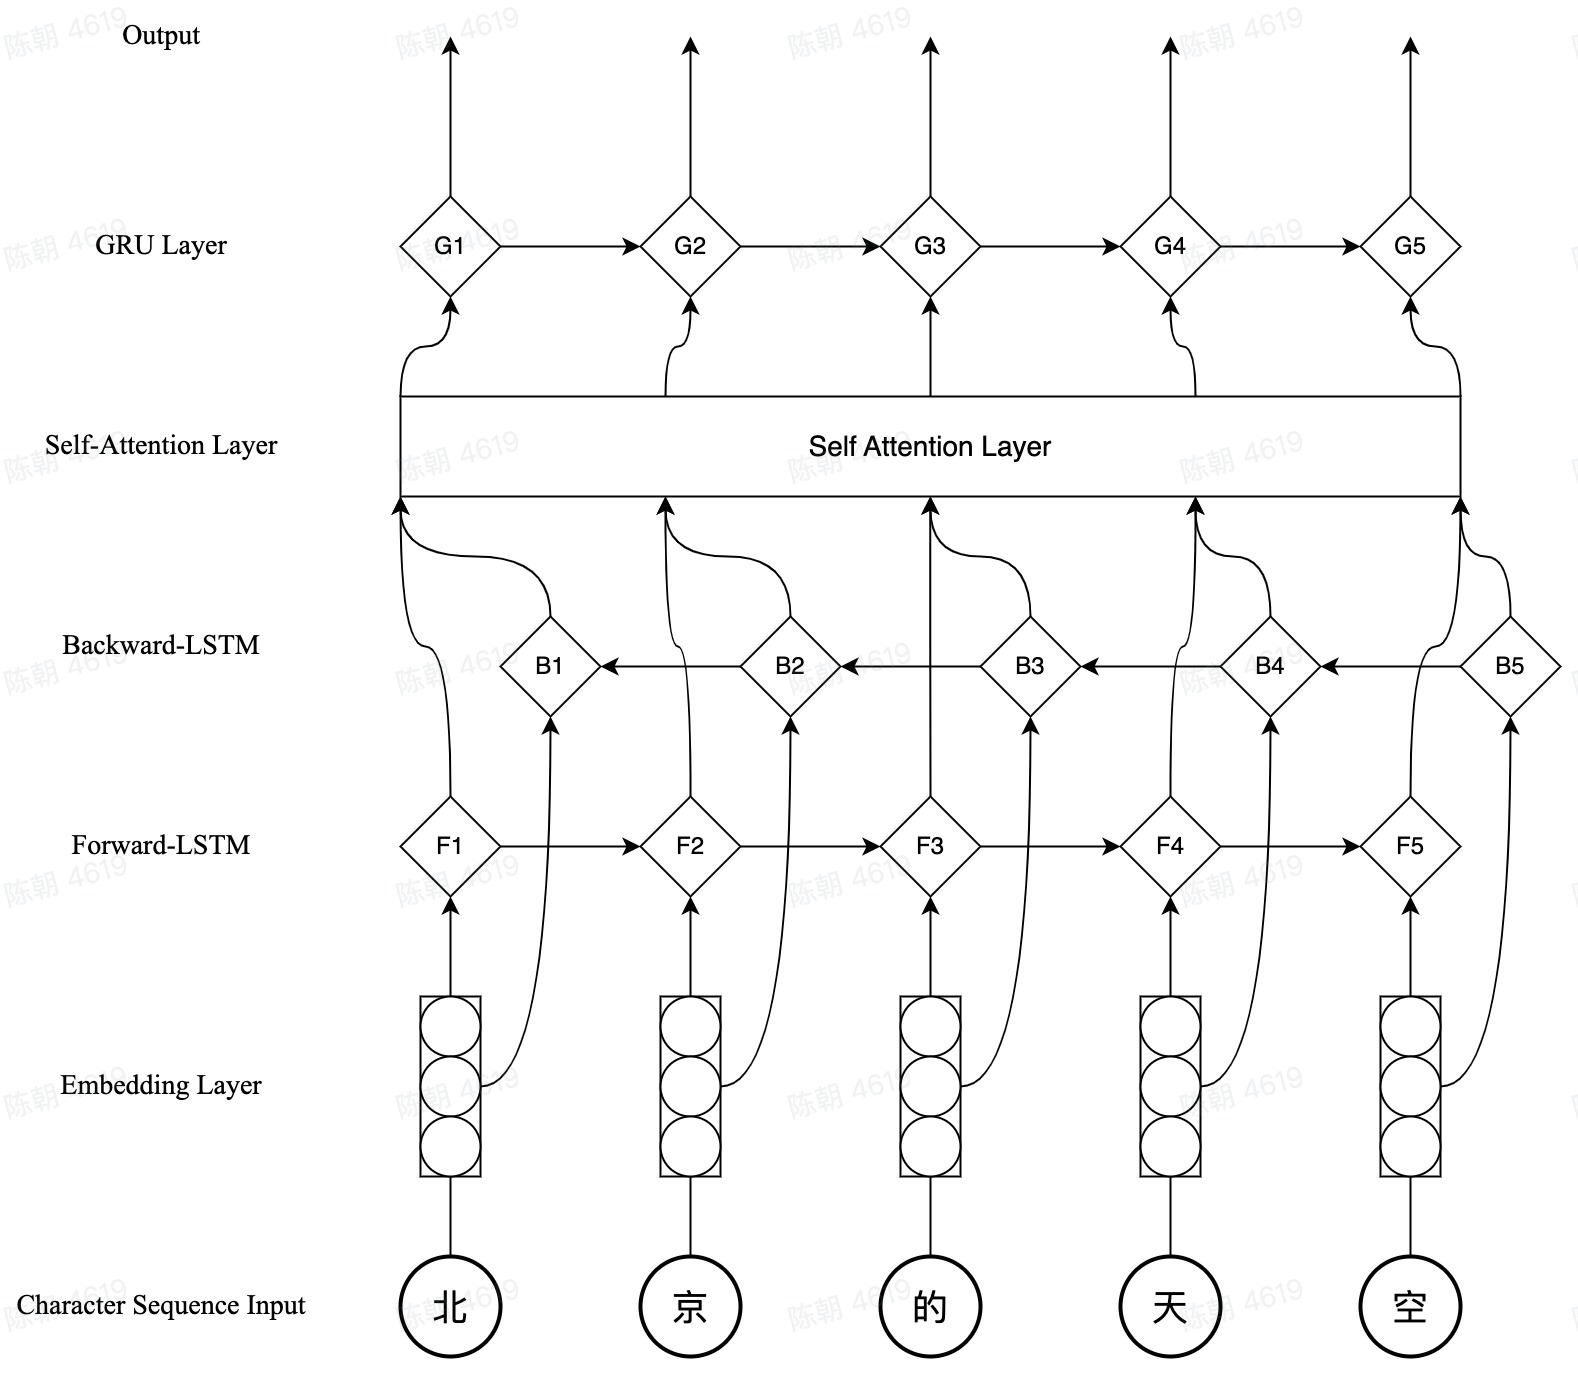
\includegraphics[width=10cm]{figures/network_architecture.jpeg}
    \caption{网络架构图}
\end{figure}

在对文本数据进行适当的预处理和字符级嵌入的基础上,将双向长短期记忆网络(BiLSTM)
和具有全局自注意层(Self-attention Layer)的门控递归单元(GRU)进行结合,
利用BiLSTM快速学习许多时间步后缓慢变化的权值,并将该权值植入GRU的自注意层里,
提出一种新的中文命名实体识别的网络架构。具体的网络结构如图~\ref{fig:network_architecture}


% \section{论文组织结构}


% 上海交通大学是我国历史最悠久的高等学府之一,是教育部直属、教育部与上海市共建的全
% 国重点大学,是国家“七五”、“八五”重点建设和“211 工程”、“985 工程”的首批建
% 设高校。经过 115 年的不懈努力,上海交通大学已经成为一所“综合性、研究型、国际化”
% 的国内一流、国际知名大学,并正在向世界一流大学稳步迈进。 

% {\songti 十九世纪末,甲午战败,民族危难。中国近代著名实业家、教育家盛宣怀和一批
%   有识之士秉持“自强首在储才,储才必先兴学”的信念,于 1896 年在上海创办了交通大
%   学的前身——南洋公学。建校伊始,学校即坚持“求实学,务实业”的宗旨,以培养“第
%   一等人才”为教育目标,精勤进取,笃行不倦,在二十世纪二三十年代已成为国内著名的
%   高等学府,被誉为“东方MIT”。抗战时期,广大师生历尽艰难,移转租界,内迁重庆,
%   坚持办学,不少学生投笔从戎,浴血沙场。解放前夕,广大师生积极投身民主革命,学校
%   被誉为“民主堡垒”。
  
%   新中国成立初期,为配合国家经济建设的需要,学校调整出相当一部分优势专业、师资设
%   备,支持国内兄弟院校的发展。五十年代中期,学校又响应国家建设大西北的号召,根据
%   国务院决定,部分迁往西安,分为交通大学上海部分和西安部分。1959 年 3月两部分同
%   时被列为全国重点大学,7 月经国务院批准分别独立建制,交通大学上海部分启用“上海
%   交通大学”校名。历经西迁、两地办学、独立办学等变迁,为构建新中国的高等教育体
%   系,促进社会主义建设做出了重要贡献。六七十年代,学校先后归属国防科工委和六机部
%   领导,积极投身国防人才培养和国防科研,为“两弹一星”和国防现代化做出了巨大贡
%   献。}

% {\heiti 改革开放以来,学校以“敢为天下先”的精神,大胆推进改革:率先组成教授代
%   表团访问美国,率先实行校内管理体制改革,率先接受海外友人巨资捐赠等,有力地推动
%   了学校的教学科研改革。1984 年,邓小平同志亲切接见了学校领导和师生代表,对学校
%   的各项改革给予了充分肯定。在国家和上海市的大力支持下,学校以“上水平、创一流”
%   为目标,以学科建设为龙头,先后恢复和兴建了理科、管理学科、生命学科、法学和人文
%   学科等。1999 年,上海农学院并入;2005 年,与上海第二医科大学强强合并。至此,学
%   校完成了综合性大学的学科布局。近年来,通过国家“985 工程”和“211 工程”的建
%   设,学校高层次人才日渐汇聚,科研实力快速提升,实现了向研究型大学的转变。与此同
%   时,学校通过与美国密西根大学等世界一流大学的合作办学,实施国际化战略取得重要突
%   破。1985 年开始闵行校区建设,历经 20 多年,已基本建设成设施完善,环境优美的现
%   代化大学校园,并已完成了办学重心向闵行校区的转移。学校现有徐汇、闵行、法华、七
%   宝和重庆南路(卢湾)5 个校区,总占地面积 4840 亩。通过一系列的改革和建设,学校
%   的各项办学指标大幅度上升,实现了跨越式发展,整体实力显著增强,为建设世界一流大
%   学奠定了坚实的基础。}

% {\ifcsname fangsong\endcsname\fangsong\else[无 \cs{fangsong} 字体。]\fi 交通大学
%   始终把人才培养作为办学的根本任务。一百多年来,学校为国家和社会培养了 20余万各
%   类优秀人才,包括一批杰出的政治家、科学家、社会活动家、实业家、工程技术专家和医
%   学专家,如江泽民、陆定一、丁关根、汪道涵、钱学森、吴文俊、徐光宪、张光斗、黄炎
%   培、邵力子、李叔同、蔡锷、邹韬奋、陈敏章、王振义、陈竺等。在中国科学院、中国工
%   程院院士中,有 200 余位交大校友;在国家 23 位“两弹一星”功臣中,有 6 位交大校
%   友;在 18 位国家最高科学技术奖获得者中,有 3 位来自交大。交大创造了中国近现代
%   发展史上的诸多“第一”:中国最早的内燃机、最早的电机、最早的中文打字机等;新中国
%   第一艘万吨轮、第一艘核潜艇、第一艘气垫船、第一艘水翼艇、自主设计的第一代战斗
%   机、第一枚运载火箭、第一颗人造卫星、第一例心脏二尖瓣分离术、第一例成功移植同种
%   原位肝手术、第一例成功抢救大面积烧伤病人手术等,都凝聚着交大师生和校友的心血智
%   慧。改革开放以来,一批年轻的校友已在世界各地、各行各业崭露头角。}

% {\ifcsname kaishu\endcsname\kaishu\else[无 \cs{kaishu} 字体。]\fi 截至 2011 年 12
%   月 31 日,学校共有 24 个学院 / 直属系(另有继续教育学院、技术学院和国际教育学
%   院),19 个直属单位,12 家附属医院,全日制本科生 16802 人、研究生24495 人(其
%   中博士研究生 5059 人);有专任教师 2979 名,其中教授 835 名;中国科学院院士 15
%   名,中国工程院院士 20 名,中组部“千人计划”49 名,“长江学者”95 名,国家杰出
%   青年基金获得者 80 名,国家重点基础研究发展计划(973 计划)首席科学家 24名,国
%   家重大科学研究计划首席科学家 9名,国家基金委创新研究群体 6 个,教育部创新团队
%   17 个。
  
%   学校现有本科专业 68 个,涵盖经济学、法学、文学、理学、工学、农学、医学、管理学
%   和艺术等九个学科门类;拥有国家级教学及人才培养基地 7 个,国家级校外实践教育基
%   地 5个,国家级实验教学示范中心 5 个,上海市实验教学示范中心 4 个;有国家级教学
%   团队 8个,上海市教学团队 15 个;有国家级教学名师 7 人,上海市教学名师 35 人;
%   有国家级精品课程 46 门,上海市精品课程 117 门;有国家级双语示范课程 7
%   门;2001、2005 和2009 年,作为第一完成单位,共获得国家级教学成果 37 项、上海市
%   教学成果 157项。}